%%%%%
% 
\documentclass[mathserif,graphics]{beamer}
\usepackage{Sweave}
\usepackage[labelformat=empty]{caption}
\mode<presentation>
\usetheme{Frankfurt} % Beamer Theme
\setbeamersize{text margin left=5mm, text margin right=5mm}
\usecolortheme{whale}
\usepackage{amsmath} % for math AMS fonts
\usepackage{centernot}
\usepackage{graphicx} % to include figures
\usepackage{subfigure} % to have figures in figures
\usepackage{multimedia} % to include movies

\usepackage[utf8]{inputenc}
\usepackage{amsfonts}
\usepackage{natbib}
\usepackage{scrpage2}
\usepackage{dsfont}
\usepackage{float}
\usepackage{amssymb}

\usepackage{bbm}

\usepackage{tikz}
\usetikzlibrary{arrows,shapes,backgrounds, patterns, decorations.markings} % loads some tikz extensions
\usepackage[english]{babel}
\useoutertheme[subsection=false]{smoothbars} % Beamer Outer Theme
\usepackage{mdframed}
\usepackage{boxedminipage}
\newcommand{\hlcolor}[2]{{\setlength{\fboxsep}{0pt}\colorbox{#1}{\strut #2}}}
\newcommand{\eg}{e.\,g. }
\newcommand{\ie}{i.\,e. }
\newcommand{\cdf}{c.\,d.\,f. }
%\usepackage[usenames,dvipsnames]{xcolor}
\definecolor{lightblue}{rgb}{0.8,0.85,1}


\defbeamertemplate*{footline}{my infolines theme}
    {
      \leavevmode%
      \hbox{%
      \begin{beamercolorbox}[wd=.44\paperwidth,ht=2.25ex,dp=1ex,center]{author
      in head/foot}%
        \usebeamerfont{author in head/foot}\insertshortauthor~~\insertshortinstitute
      \end{beamercolorbox}%
      \begin{beamercolorbox}[wd=.2\paperwidth,ht=2.25ex,dp=1ex,center]{title in
      head/foot}%
        \usebeamerfont{title in head/foot}\insertshorttitle
      \end{beamercolorbox}%
      \begin{beamercolorbox}[wd=.36\paperwidth,ht=2.25ex,dp=1ex,right]{date in
      head/foot}%
        \usebeamerfont{date in head/foot}\insertshortdate{}\hspace*{2em}
        \insertframenumber{} / \inserttotalframenumber\hspace*{2ex}
      \end{beamercolorbox}}%
      \vskip0pt%
    }

\title{Normal Distribution}
%\subtitle{Seminar graph algorithms}
\author{Andrey Chinnov, Sebastian Honermann, Carlos Zydorek}
%\institute{Seminar graph algorithms}
\date{Case Studies \\
"Data Analytics"}

\begin{document}
\frame{
\titlepage
\setbeamercovered{dynamic}
}



\section{Introduction}
\frame{
\frametitle{Outline}
\begin{enumerate}
\item \alert {Introduction}
  \begin{itemize}
  \item Normality as a requirement for statistical methods
  \item Data Set Overview
  \end{itemize}
\item Normality Testing
  \begin{itemize}
  \item Graphical Methods for Normality Testing
    \begin{itemize}
    \item Q-Q-Plots
    \item Chi-Square Plot
    \end{itemize}
  \item Quantitative Methods for Normality Testing
    \begin{itemize}
    \item Shapiro-Wilk Test
    \item Pearson's Chi-Squared Test
    \item Kolmogorov-Smirnov Test
    \end{itemize}
  \end{itemize}
\item Transformation to Normality
  \begin{itemize}
  \item Box-Cox Transformation
  \item Transformation Results Testing 
  \end{itemize}
\item Summary
\end{enumerate}
}
\subsection{Normality as a requirement for statistical methods}

\frame{
\frametitle{Normality as a requirement for statistical methods}

}

\subsection{Data Set Overview}

\frame{
\frametitle{Data Set Overview}

}

\section{Normality Testing}
\frame{
\frametitle{Outline}
\begin{enumerate}
\item Introduction
  \begin{itemize}
  \item Normality as a requirement for statistical methods
  \item Data Set Overview
  \end{itemize}
\item \alert{Normality Testing}
  \begin{itemize}
  \item Graphical Methods for Normality Testing
    \begin{itemize}
    \item Q-Q-Plots
    \item Chi-Square Plot
    \end{itemize}
  \item Quantitative Methods for Normality Testing
    \begin{itemize}
    \item Shapiro-Wilk Test
    \item Pearson's Chi-Squared Test
    \item Kolmogorov-Smirnov Test
    \end{itemize}
  \end{itemize}
\item Transformation to Normality
  \begin{itemize}
  \item Box-Cox Transformation
  \item Transformation Results Testing 
  \end{itemize}
\item Summary
\end{enumerate}
}

\subsection{Q-Q-Plots}
\frame{
\frametitle{Q-Q-Plots}
\footnotesize
\begin{columns}[t]
\column{0.3\columnwidth}
{\bf Sample:}
\[x=(x_1,x_2,\dots,x_n)\]
{\bf Empirical quantiles:}
\[x_{(1)}\le x_{(2)} \le \dots \le x_{(n)}\]
{\bf Theoretical quantiles:}
\[q_{(j)} = \Phi^{-1}(p_{(j)}),\]
where
\[ p_{(j)} = \frac{j - \frac{1}{2}} {n},\]
\[\Phi\mbox{ - }N(0,1)\mbox{ \cdf.}\]

\[\implies \mbox{ Plot } x_{(i)}\mbox{ against } q_{(i)}\]
\vspace{15cm}
\column{0.7\columnwidth}
\vspace{-1.35cm}
\begin{figure}
	\includegraphics[width=\columnwidth]{report-QQfull}
	\end{figure}
\end{columns}
\vspace{15cm}
}

\frame{
\frametitle{Q-Q-Plots}
\footnotesize
\begin{columns}[t]
\column{0.4\columnwidth}
\centerline{{\bf QQ-Plots of the subdatasets:}}

\begin{itemize}
\item Variables could be normally distributed within the subclasses 
\item For some cases there appear to be a linear relationships
\item For other cases a linear relationship is questionable
\item In some subdatasets a linear relationship seems plausible, however $n$ is very small
\end{itemize}
\vspace{15cm}
\column{0.6\columnwidth}
\vspace{-1cm}
\begin{figure}
	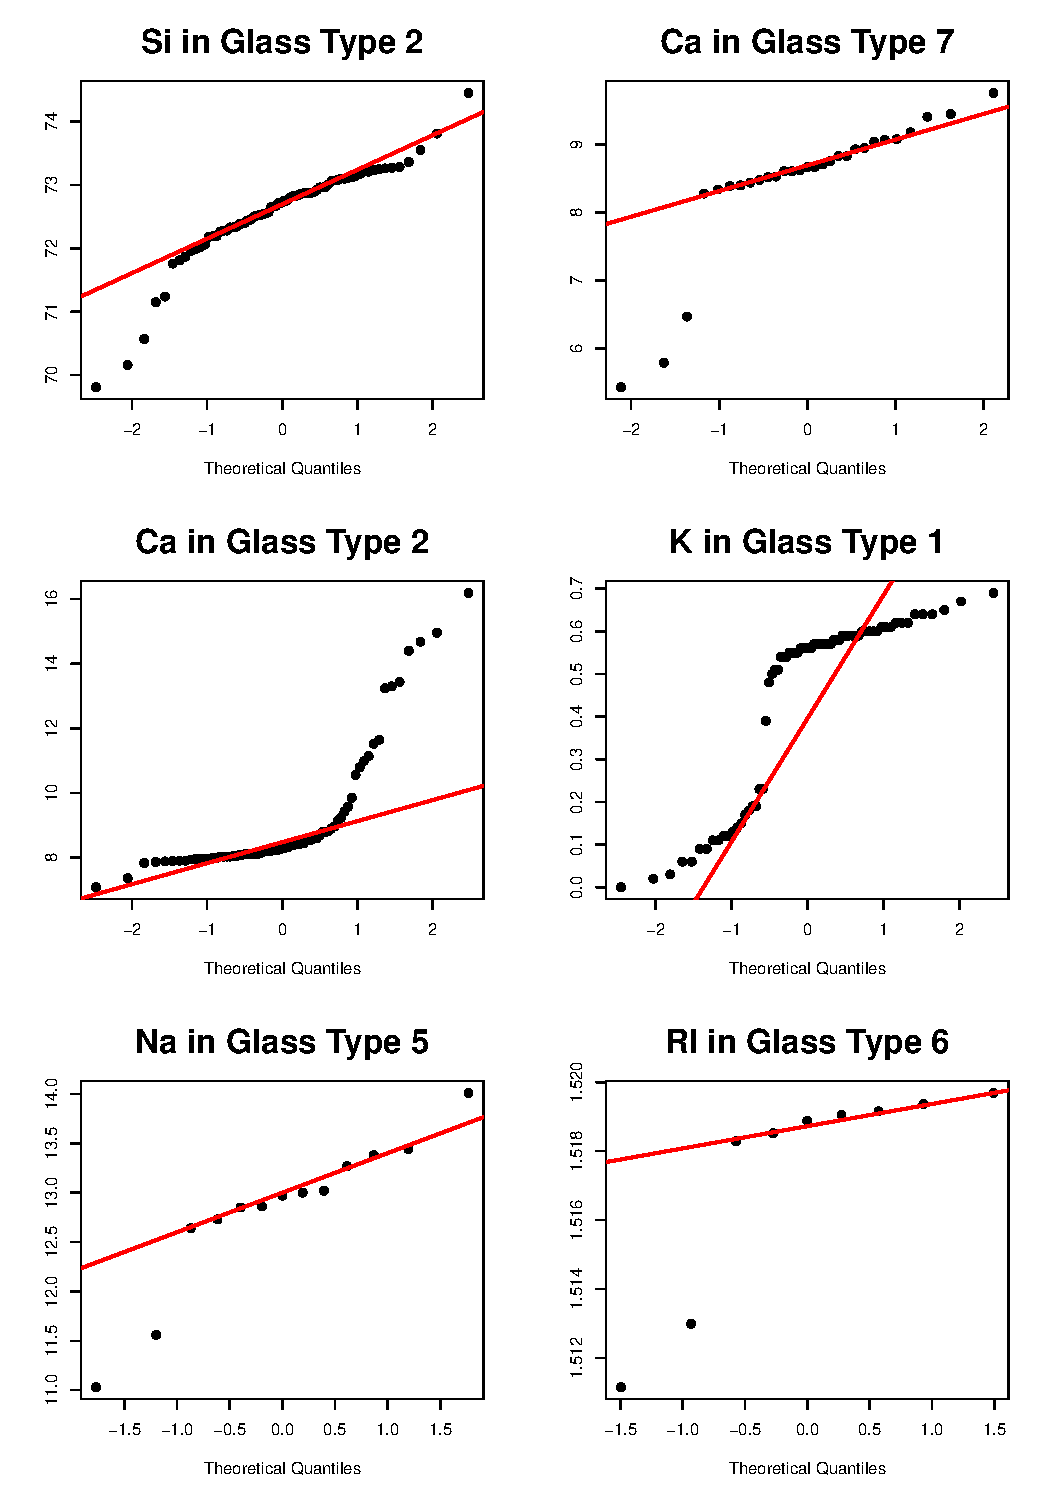
\includegraphics[width=0.8\columnwidth]{graph}
	\end{figure}
\end{columns}
\vspace{15cm}
}

\frame{
\frametitle{Q-Q-Plots}
\footnotesize
\begin{columns}[t]
\column{0.4\columnwidth}
\begin{center}
{\bf Results of the Transformation of the Full Dataset
:}
\end{center}

\begin{itemize}
\item For some of the cases there seems to be a slight improvement

\item For non-unimodal cases the transformation does not show significant improvements towards normality
\end{itemize}
\vspace{15cm}
\column{0.6\columnwidth}
\vspace{-1cm}
\begin{figure}
	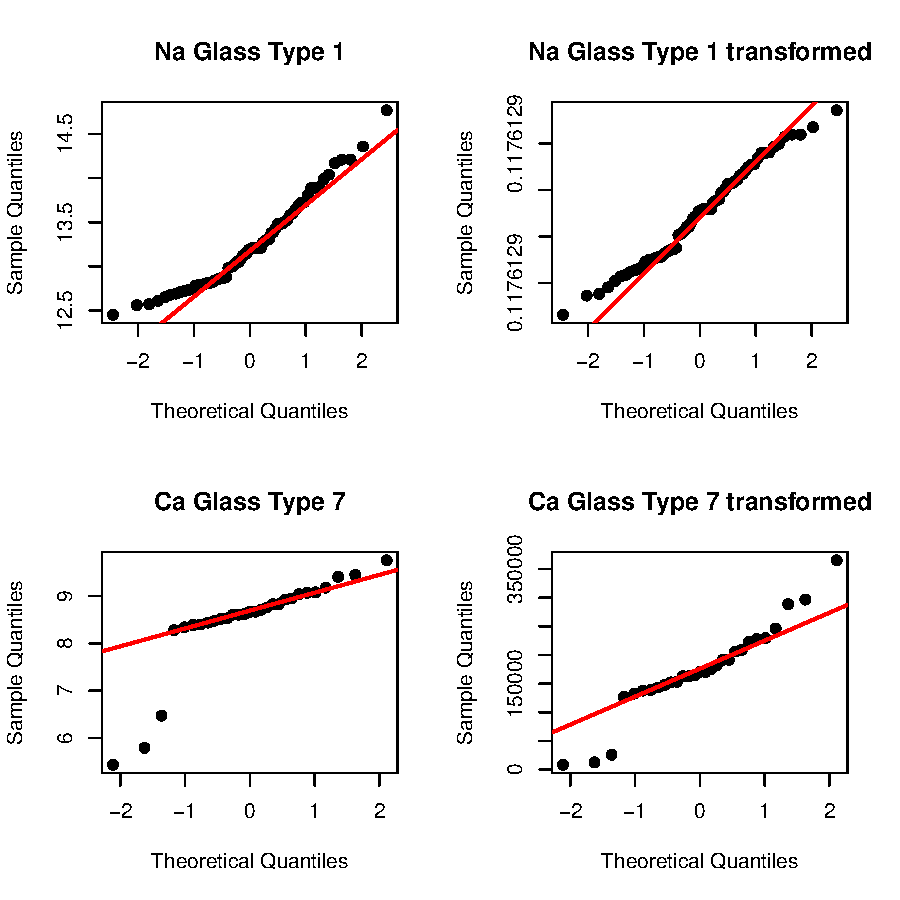
\includegraphics[width=\columnwidth]{Report-QQtrans}
	\end{figure}
\end{columns}
\vspace{15cm}
}

\frame{
\frametitle{Q-Q-Plots}
\footnotesize
\begin{columns}[t]
\column{0.4\columnwidth}
\begin{center}
{\bf Results of the Transformation of the Subdatasets
:}
\end{center}

\begin{itemize}
\item For unimodal cases the transformation shapes the distribution closer to normality

\item For non-unimodal cases the transformation does not show significant improvements towards normality
\end{itemize}
\vspace{15cm}
\column{0.6\columnwidth}
\vspace{-1cm}
\begin{figure}
	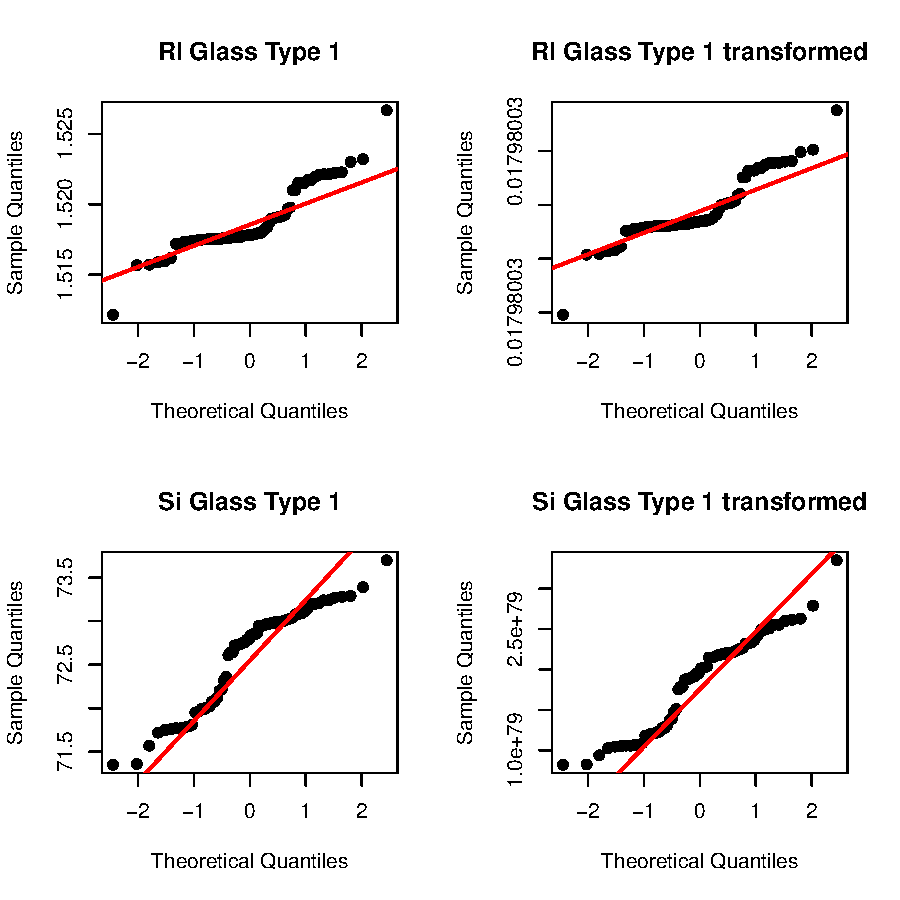
\includegraphics[width=\columnwidth]{Report-QQtransno}
	\end{figure}
\end{columns}
\vspace{15cm}
}

\subsection{Shapiro-Wilk Test}
\frame{
\frametitle{Shapiro-Wilk Test}
The test statistic $W$ indicates the deviation of the observed quantile values from the assumed cumulative distribution function quantiles 
\[W = \frac{\sum  \limits_{i=1}^n(a_i y_i)^2}{\sum  \limits_{i=1}^n (y_i-\bar{y})^2},\]
where
\begin{itemize}
\item $a_i$ denotes the normalised "best linear unbiased" coefficients,
\item $y_i$ denotes the observations.
\end{itemize}

The critical value for $W$ is obtained by the Monte Carlo Method\\
$\implies$ $p$-value is calculated

\alert{Important:} If a variable contains only zeros the Shapiro-Wilk test is not applicable, 
since the term in the denominator sums up to zero.
}

\frame{
\frametitle{Shapiro-Wilk Test}
\begin{columns}[t]
\column{0.23\columnwidth}
\scriptsize
\vspace{-0.5cm}
\begin{center}
{\bf Testing the Full Dataset
:}
\end{center}
Null hypothesis is rejected for all variables at a 1 \% significance level
\begin{center}
{\bf After the Transformation
:}
\end{center}

The null hypothesis can be rejected for the four transformed variables

\alert{$\implies$ Possible Explanation:} Combination of different 	
distributions in the different glass types
\vspace{15cm}
\column{0.77\columnwidth}
\tiny
\vspace{-0.8cm}
\begin{table}[h!]
\centering
\begin{tabular}{|cccccc|} \hline variable & test statistic & sig. level & critical value & p-value & rejected\\ \hline RI & 0.87 & 0.01 & NA & 1.0766713449726e-12 & yes\\ 
Na & 0.95 & 0.01 & NA & 3.4655430546966e-07 & yes\\ 
Mg & 0.7 & 0.01 & NA & < 1.0e-15 & yes\\ 
Al & 0.94 & 0.01 & NA & 2.08315629600399e-07 & yes\\ 
Si & 0.92 & 0.01 & NA & 2.17503176825416e-09 & yes\\ 
K & 0.44 & 0.01 & NA & < 1.0e-15 & yes\\ 
Ca & 0.79 & 0.01 & NA & < 1.0e-15 & yes\\ 
Ba & 0.41 & 0.01 & NA & < 1.0e-15 & yes\\ 
Fe & 0.65 & 0.01 & NA & < 1.0e-15 & yes\\ \hline \end{tabular}
\caption{\scriptsize Test results of the Shapiro-Wilk test on the whole
data sample}
\end{table}
\vspace{-1cm}
\begin{table}[h!]
\centering
\begin{tabular}{|cccccc|} \hline variable & test statistic & sig. level & critical value & p-value & rejected\\ \hline RI & NA & NA & NA & NA & NA\\ 
Na & 0.95 & 0.01 & NA & 8.75605777309153e-07 & yes\\ 
Mg & NA & NA & NA & NA & NA\\ 
Al & 0.97 & 0.01 & NA & 0.000244326513056066 & yes\\ 
Si & 0.93 & 0.01 & NA & 1.58998125691823e-08 & yes\\ 
K & NA & NA & NA & NA & NA\\ 
Ca & 0.89 & 0.01 & NA & 1.13880689831982e-11 & yes\\ 
Ba & NA & NA & NA & NA & NA\\ 
Fe & NA & NA & NA & NA & NA\\ \hline \end{tabular}
\caption{\scriptsize Test results of the Shapiro-Wilk test on the whole
transformed data sample}
\end{table}
\vspace{15cm}
\end{columns}
}

\frame{
\frametitle{Shapiro-Wilk Test}
\begin{columns}[t]
\column{0.23\columnwidth}
\scriptsize
\vspace{-0.5cm}

{\bf Testing the Subdatasets Example – Glass Type 1
:}\\
\vspace{0.25cm}
Null hypothesis is rejected for all variables at a 1 \% significance level\\
\vspace{0.5cm}

{\bf After the Transformation
:}\\
\vspace{0.25cm}
The null hypothesis cannot be rejected for 3 of the transformed variables\\
\vspace{0.3cm}
\alert{$\implies$} 
Appearently the 	transformation was 	successful
\vspace{15cm}
\column{0.77\columnwidth}
\tiny
\vspace{-0.8cm}
\begin{table}[h!]
\centering
\begin{tabular}{|cccccc|} \hline variable & test statistic & sig. level & critical value & p-value & rejected\\ \hline RI & 0.88 & 0.01 & NA & 6.36192013015468e-06 & yes\\ 
Na & 0.95 & 0.01 & NA & 0.00459078607995831 & yes\\ 
Mg & 0.82 & 0.01 & NA & 8.02702432879544e-08 & yes\\ 
Al & 0.9 & 0.01 & NA & 5.42971629496434e-05 & yes\\ 
Si & 0.91 & 0.01 & NA & 0.000117060780025464 & yes\\ 
K & 0.77 & 0.01 & NA & 3.14049093233846e-09 & yes\\ 
Ca & 0.93 & 0.01 & NA & 0.00103561283726753 & yes\\ \hline \end{tabular}
\caption{\scriptsize Test results of the Shapiro-Wilk test on type 1 glass}
\end{table}
\begin{table}[h!]
\centering
\begin{tabular}{|cccccc|} \hline variable & test statistic & sig. level & critical value & p-value & rejected\\ \hline RI & 0.89 & 0.01 & NA & 1.62433657125306e-05 & yes\\ 
Na & 0.98 & 0.01 & NA & 0.353792914291578 & no\\ 
Mg & 0.83 & 0.01 & NA & 1.40023833110547e-07 & yes\\ 
Al & 0.96 & 0.01 & NA & 0.0459207068393172 & no\\ 
Si & 0.94 & 0.01 & NA & 0.00269629206710463 & yes\\ 
K & NA & NA & NA & NA & NA\\ 
Ca & 0.97 & 0.01 & NA & 0.148237775100495 & no\\ \hline \end{tabular}
\caption{\scriptsize Test results of the Shapiro-Wilk test on the transformed
type 1 glass}
\end{table}
\vspace{15cm}
\end{columns}
}

\subsection{Chi-Square Plot}
\frame{
\frametitle{Graphical Methods for Normality Testing}
\framesubtitle{Chi-Square Plot}
}

\subsection{Pearson's Chi-Squared Test}
\frame{
\frametitle{Quantitative Methods for Normality Testing}
\framesubtitle{Pearson's Chi-Squared Test}
}

\subsection{Kolmogorov-Smirnov Test}
\frame{
\frametitle{Quantitative Methods for Normality Testing}
\framesubtitle{Kolmogorov-Smirnov Test}
Let $x=(x_1,x_2, \dots, x_n)$ be a sample of unknown
distribution $\mathbb{P}$.
\begin{columns}[t]
\column{0.5\columnwidth}
\begin{definition}
$F_n(x)=\frac{1}{n}\sum_{i=1}^n \mathbbm{1}_{\{x_i\le x\}}(x)$ \\
- \alert{empirical} \cdf, where \\
$\mathbbm{1}_{\{x_i\le x\}}(x)=\left\lbrace 
\begin{array}{cll}
                1 & \mbox{if} \ x_i\le x\\
                 0 & \mbox{otherwise}.
\end{array} 
\right.$
\end{definition}
\onslide<2->{
$F(x)$ - theoretical normal \cdf with
\[\bar{x}=\frac{1}{n}\sum_i x_i,\quad \sigma^2_x=\frac{1}{n}(x_i-\bar{x})^2\]}
\onslide<3->{
$d=\sup_{x\in \mathbb{R}}|F_n(x)-F(x)|$ \\- distance between them.}
\column{0.5\columnwidth}
  \vspace{-1cm}
    \only<1>{
    \begin{figure}
	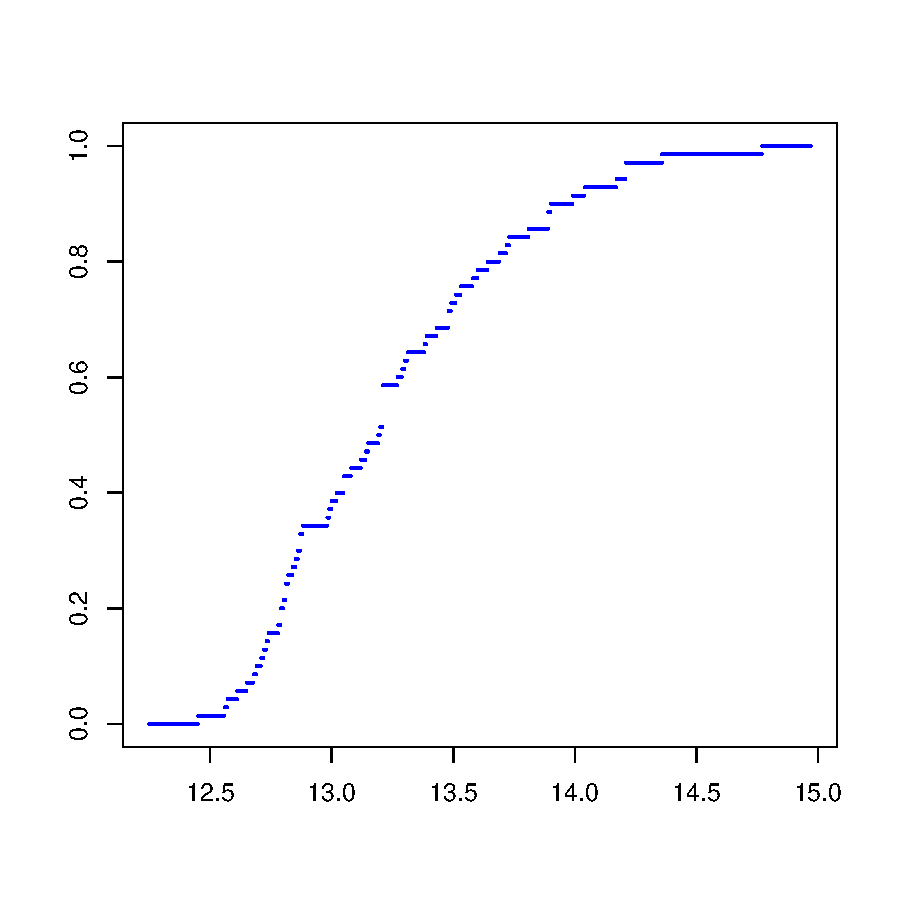
\includegraphics[width=\columnwidth]{Report-empiricFunc}
	\end{figure}}
    \only<2->{
    \begin{figure}
	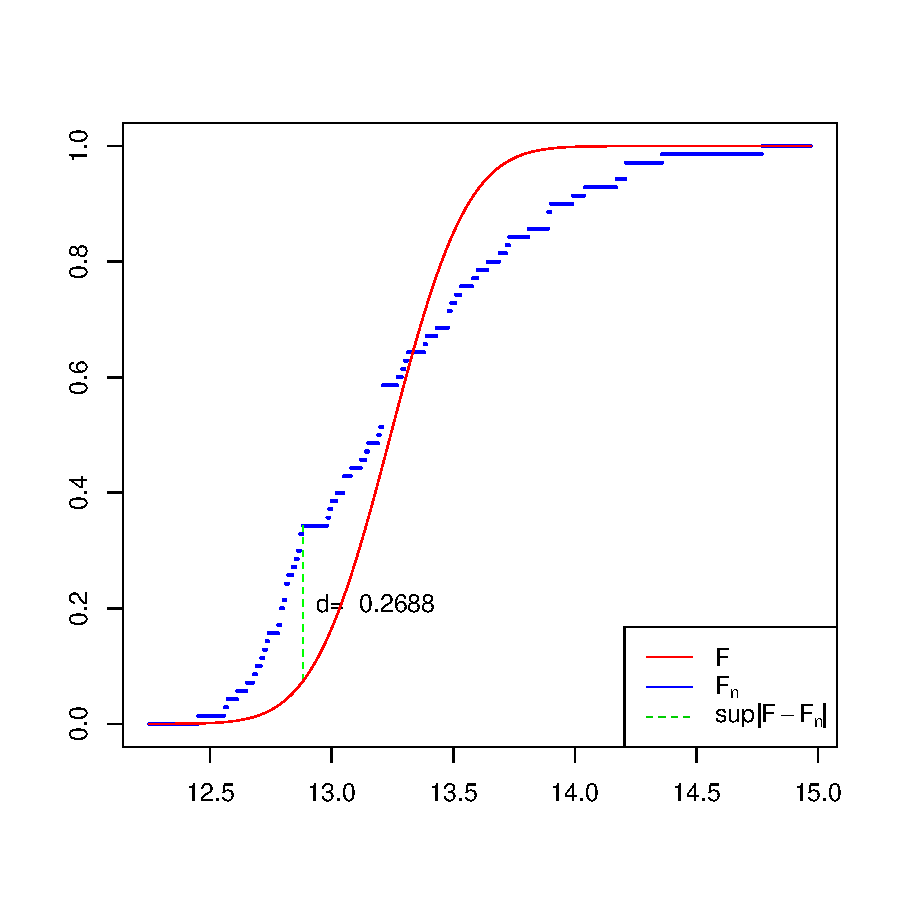
\includegraphics[width=\columnwidth]{Report-empiricTeorFunc}
	\end{figure}}
\vspace{-1.5cm}
\begin{center}
Glass Type 1, Natrium (Na)
\end{center}
\end{columns}
}

\frame{
\frametitle{Quantitative Methods for Normality Testing}
\framesubtitle{Kolmogorov-Smirnov Test}
Let $x=(x_1,x_2, \dots, x_n)$ be a sample of unknown
distribution $\mathbb{P}$.\\
Theoretical \cdf $F$ defines a distribution $\mathbb{P}_0$.\\
\onslide<2->{
\[\begin{array}{rcl}
H_0 & : & \mathbb{P} = \mathbb{P}_0,\\
H_1 & : & \mathbb{P} \ne \mathbb{P}_0.
\end{array}\]}
\onslide<3->{
KS test statistics:
\[D_n = \sqrt{n}\cdot \sup_{x \in \mathbb{R}}|F_n(x)-F(x)|.\]}
\onslide<4->{
Properties of $D_n$ in case $H_0$ is \alert{TRUE}:}
\begin{itemize}
\item<4-> Distribution of $\hat{D}_n:=(D_1,D_2,\dots, D_n)$ does not depend on
$F$\\
\onslide<5->{\hfill$\implies$ \alert{tabulated}}
\item<6-> $\forall t>0:$ \[P(D_n\le t)\xrightarrow[n \to \infty]{}
H(t)=1-2\sum_{i=1}^{\infty}(-1)^{i-1} \exp^{-2i^2t^2}\]
\end{itemize}

\vspace{15cm}
}

\frame{
\frametitle{Quantitative Methods for Normality Testing}
\framesubtitle{Kolmogorov-Smirnov Test}
The KS test uses the decision rule
\[ \delta = 
\left\{
\begin{array}{rcl}
H_0&:& D_n\le c\\
H_1&:& D_n> c
\end{array}
\right.,
\]
where $c$ - critical value \onslide<2-> {that\\
depends on a significance level $\alpha$:}
\[\onslide<3->{\alpha = P(\delta \ne H_0|H_0)}\onslide<4->{=P(D_n>c|H_0)}\onslide<5->{=1-P(D_n\le c|H_0)}\onslide<6->{\approx 1-H(c).}\]
\onslide<7->{\[\implies \alert{c\approx H_{1-\alpha}}\]}

\vspace{15cm}
}

\frame{
\frametitle{Quantitative Methods for Normality Testing}
\framesubtitle{Kolmogorov-Smirnov Test}
The KS test uses the decision rule for a given significance level $\alpha$
\[ \delta = 
\left\{
\begin{array}{rcl}
H_0&:& D_n\le H_{1-\alpha}\\
H_1&:& D_n> H_{1-\alpha}
\end{array}
\right., \quad H(t)=1-2\sum_{i=1}^{\infty}(-1)^{i-1} \exp^{-2i^2t^2}
\]
\begin{columns}[t]
\column{0.5\columnwidth}
\onslide<2->{\centerline{{\bf Example:}}}\\
\begin{itemize}
\item<3->
$n=70$
\item<4->
$D_n=\sqrt{n}
\sup|F_n-F|=2.2493$
\item<5->
$\alpha = 0.01$\\
\hfill$\implies
c=H_{1-\alpha}=1.6276$

\item<6->
$D_n>c \implies  H_0$ \alert{rejected}

\item<7-> 
$\implies \mathbb{P}\ne \mathbb{P}_0$

\item<8-> \alert{$\centernot\implies$
 data not normally distributed!!!}
\end{itemize}

\column{0.5\columnwidth}
  \vspace{-1.9cm}
    \onslide<2->{
    \begin{figure}
	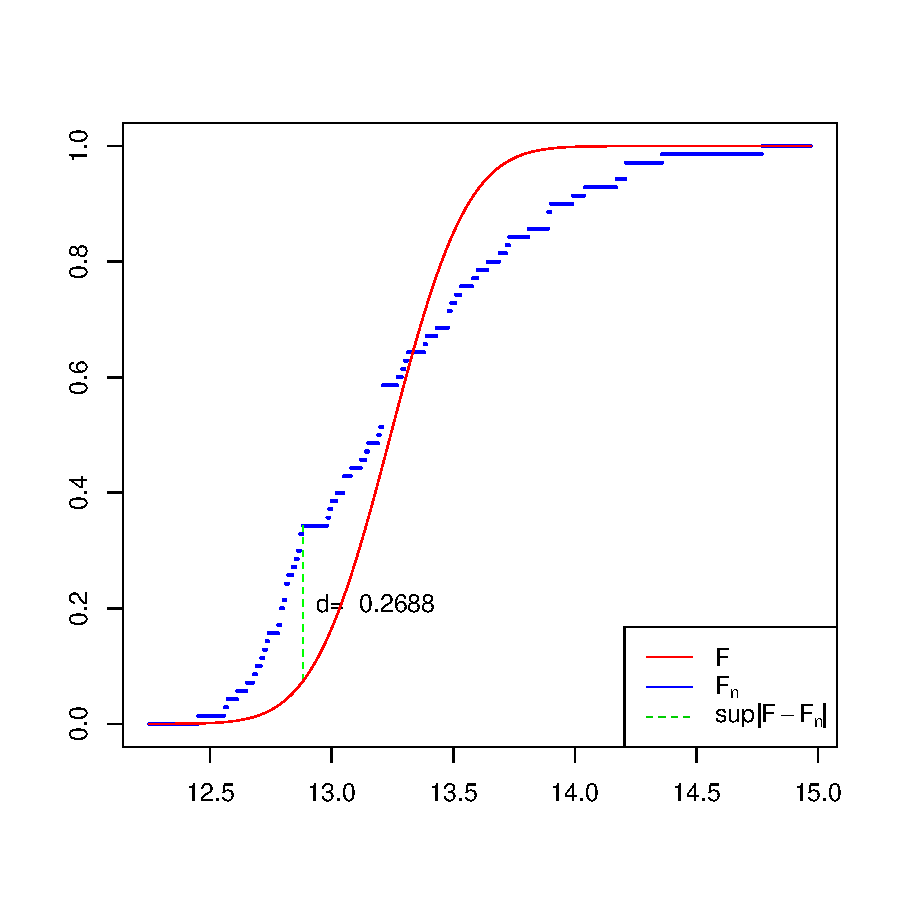
\includegraphics[width=\columnwidth]{Report-empiricTeorFunc}
	\end{figure}
\vspace{-1.5cm}
\begin{center}
Glass Type 1, Natrium (Na)
\end{center}}
\end{columns}

\vspace{15cm}
}

\begin{frame}[fragile]
\frametitle{Quantitative Methods for Normality Testing}
\framesubtitle{Improved Kolmogorov-Smirnov Test}
KS test is improved by solving the following
optimization problem \[KS(\mu,\sigma)=\sup_{x \in
\mathbb{R}}|F_n(x)-F(x,\mu,\sigma)|\to \min.\]
\begin{itemize}
\item<1->[]$R$ code used:
\item<2->[]
\begin{Schunk}
\begin{Sinput}
 c(mean(dat),var(dat))
\end{Sinput}
\begin{Soutput}
[1] 13.2422857  0.2493019
\end{Soutput}
\begin{Sinput}
 #optim is a predifined R function in stats package
 #defalut method of optimization is Nelder and Mead
 result = optim(c(mean(dat),var(dat)),KS)
 result$par
\end{Sinput}
\begin{Soutput}
[1] 13.1769501  0.4682486
\end{Soutput}
\begin{Sinput}
 result$value
\end{Sinput}
\begin{Soutput}
[1] 0.07870673
\end{Soutput}
\end{Schunk}
\end{itemize}
\vspace{10cm}
\end{frame}


\frame{
\frametitle{Quantitative Methods for Normality Testing}
\framesubtitle{Improved Kolmogorov-Smirnov Test}
KS test is improved by solving the following
optimization problem \[KS(\mu,\sigma)=\sup_{x \in
\mathbb{R}}|F_n(x)-F(x,\mu,\sigma)|\to \min.\]
\begin{columns}[t]
\column{0.5\columnwidth}
\vspace{-1cm}
\begin{itemize}
\item<1->Initial vector of parameters
$\mu=13.2423,\quad
\sigma^2=0.2493$
\item<1->Optimized vector of parameters
$\hat{\mu}=13.1770, \quad
\hat{\sigma}^2=0.4682$
\item<3->
$D_n=\sqrt{n}
\sup|F_n-F_{new}|=0.6585$
\item<4->
$c=1.6276$
\item<5->
$D_n<c \implies  H_0$ \alert{accepted}

\item<6-> 
$\implies \mathbb{P}= \mathbb{P}_0$

\item<7-> \alert{$\implies$
 data normally distributed!}
\end{itemize}

\column{0.5\columnwidth}
  \vspace{-1.9cm}
    \only<1>{
    \begin{figure}
	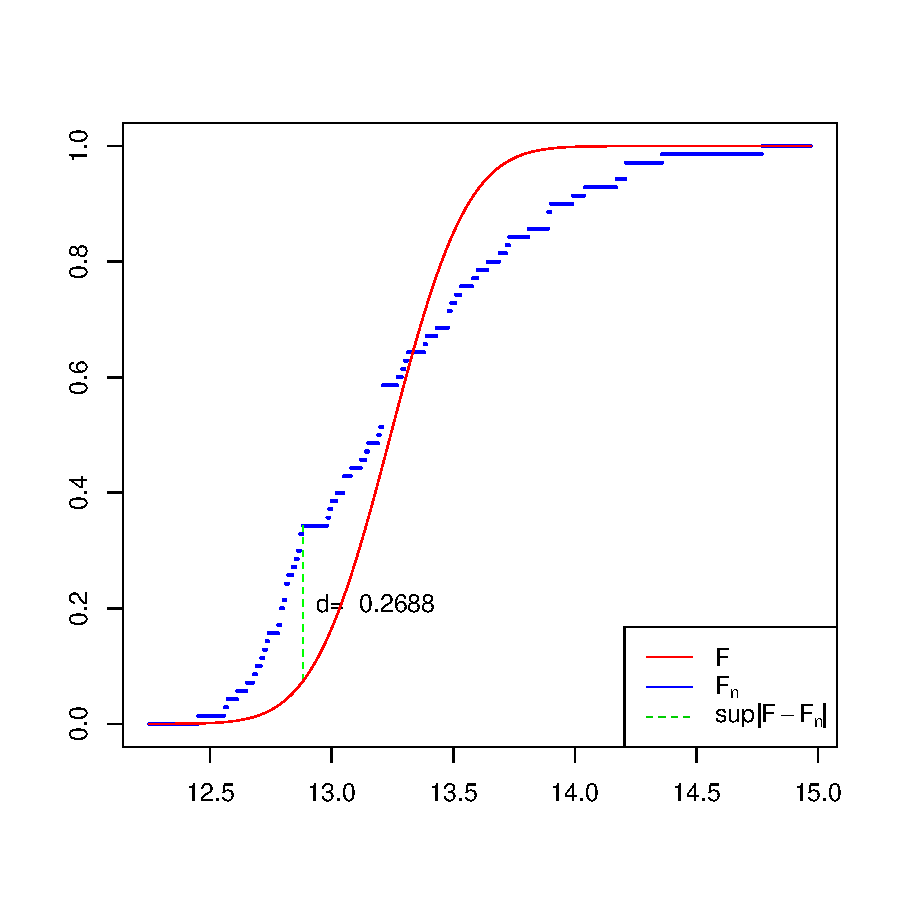
\includegraphics[width=\columnwidth]{Report-empiricTeorFunc}
	\end{figure}}
    \only<2->{
    \begin{figure}
	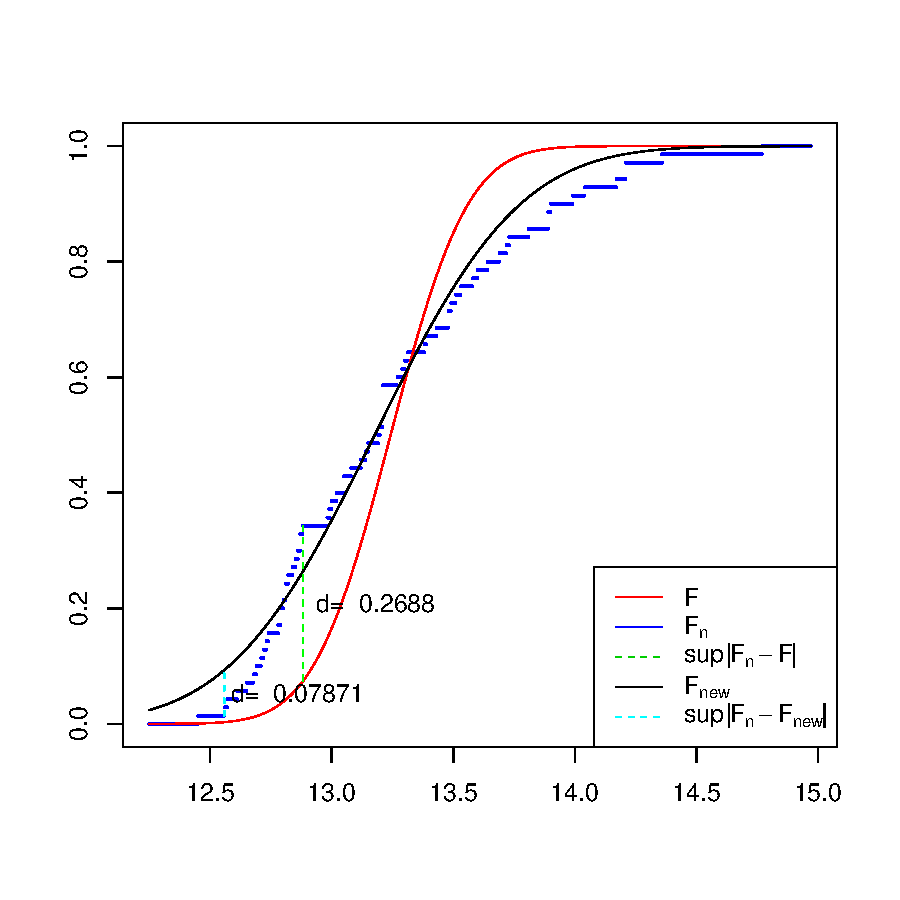
\includegraphics[width=\columnwidth]{Report-improvedKS}
	\end{figure}}
\onslide<2->{
\vspace{-1.5cm}
\begin{center}
Glass Type 1, Natrium (Na)
\end{center}}
\end{columns}

\vspace{15cm}
}


\frame{
\frametitle{Quantitative Methods for Normality Testing}
\framesubtitle{Improved Kolmogorov-Smirnov Test Results}
Results of Improved KS test on the whole data set:
\scriptsize
\begin{table}[h!]
\centering
\begin{tabular}{|cccccc|} \hline variable & test statistic & sig. level & critical value & p-value & rejected\\ \hline RI & 1.34 & 0.01 & 1.63 & 0.0561963016778131 & no\\ 
Na & 0.87 & 0.01 & 1.63 & 0.43825271603342 & no\\ 
Mg & 2.94 & 0.01 & 1.63 & 6.18457917100912e-08 & yes\\ 
Al & 0.84 & 0.01 & 1.63 & 0.474757887353829 & no\\ 
Si & 0.96 & 0.01 & 1.63 & 0.314710019077325 & no\\ 
K & 2.14 & 0.01 & 1.63 & 0.000212776619708754 & yes\\ 
Ca & 1.33 & 0.01 & 1.63 & 0.057710602872685 & no\\ 
Ba & 2.60 & 0.01 & 1.63 & 2.75476085742632e-06 & yes\\ 
Fe & 4.68 & 0.01 & 1.63 & < 1.0e-15 & yes\\ \hline \end{tabular}
\end{table}
\normalsize
\begin{itemize}
\item<2-> 5 variables are normaly distributed (RI,Na,Al,Si,Ca)
\item<3-> 4 variables are not (Mg,K,Ba,Fe)
\item<4-> The best statistics test value for Al
\item<5-> The worst statistic test value for Fe
\end{itemize}
\vspace{15cm}
}

\frame{
\frametitle{Quantitative Methods for Normality Testing}
\begin{columns}[t]
\column{0.3\columnwidth}

{\bf \centerline{Test Results:}}
\begin{table}[h!]
\centering
\begin{tabular}{|cc|} \hline variable & rejected\\ 
\hline 
RI & no\\ 
Na & no\\ 
Mg & yes\\ 
Al & no\\ 
Si & no\\ 
K & yes\\ 
Ca & no\\ 
Ba & yes\\ 
Fe & yes\\ 
\hline 
\end{tabular}
\end{table}

\column{0.7\columnwidth}
\only<2->{
\vspace{-1.35cm}
\begin{figure}
	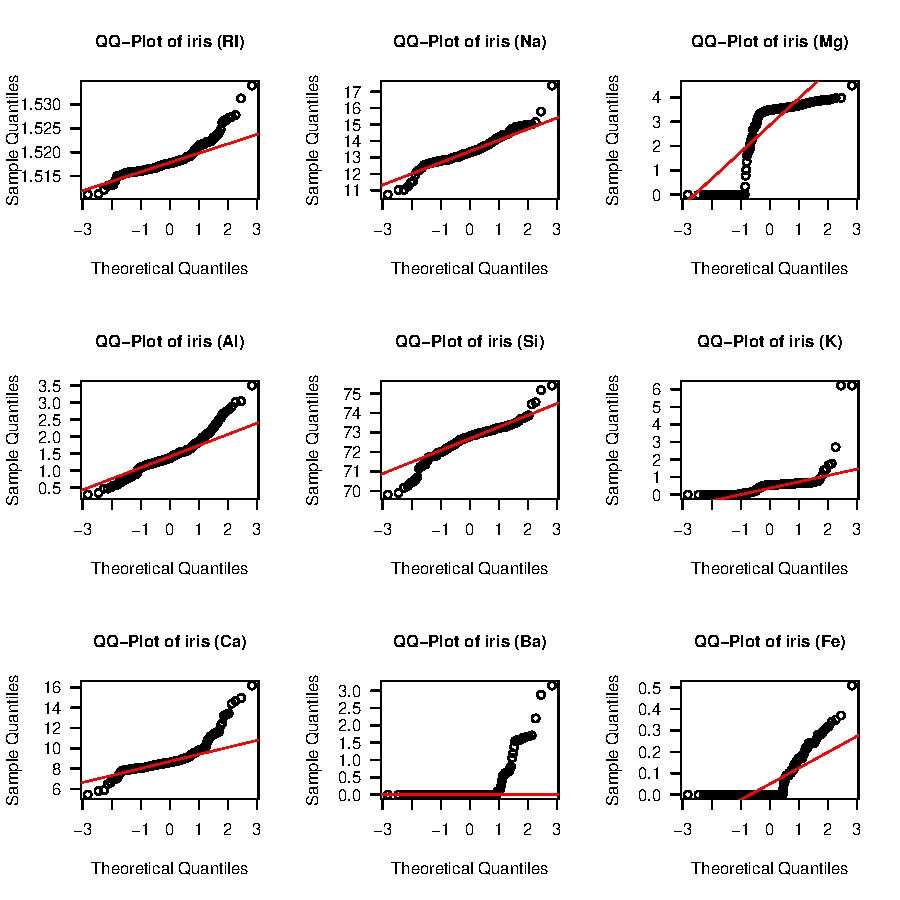
\includegraphics[width=\columnwidth]{auxiliary-drawQQPlots}
	\end{figure}}
\end{columns}
\vspace{15cm}
}

\section{Transformation to Normality}
\frame{
\frametitle{Outline}
\begin{enumerate}
\item Introduction
  \begin{itemize}
  \item Normality as a requirement for statistical methods
  \item Data Set Overview
  \end{itemize}
\item Normality Testing
  \begin{itemize}
  \item Graphical Methods for Normality Testing
    \begin{itemize}
    \item Q-Q-Plots
    \item Chi-Square Plot
    \end{itemize}
  \item Quantitative Methods for Normality Testing
    \begin{itemize}
    \item Shapiro-Wilk Test
    \item Pearson's Chi-Squared Test
    \item Kolmogorov-Smirnov Test
    \end{itemize}
  \end{itemize}
\item \alert{Transformation to Normality}
  \begin{itemize}
  \item Box-Cox Transformation
  \item Transformation Results Testing 
  \end{itemize}
\item Summary
\end{enumerate}
}
\subsection{Box-Cox Transformation}

\frame{
\frametitle{Box-Cox Transformation}

}

\subsection{Transformation Results Testing}

\frame{
\frametitle{Transformation Results Testing}

}

\section{Summary}
\frame{
\frametitle{Outline}
\begin{enumerate}
\item Introduction
  \begin{itemize}
  \item Normality as a requirement for statistical methods
  \item Data Set Overview
  \end{itemize}
\item Normality Testing
  \begin{itemize}
  \item Graphical Methods for Normality Testing
    \begin{itemize}
    \item Q-Q-Plots
    \item Chi-Square Plot
    \end{itemize}
  \item Quantitative Methods for Normality Testing
    \begin{itemize}
    \item Shapiro-Wilk Test
    \item Pearson's Chi-Squared Test
    \item Kolmogorov-Smirnov Test
    \end{itemize}
  \end{itemize}
\item Transformation to Normality
  \begin{itemize}
  \item Box-Cox Transformation
  \item Transformation Results Testing 
  \end{itemize}
\item \alert{Summary}
\end{enumerate}
}
\subsection{Summary}
\frame{
\frametitle{Summary}
}

\end{document}
